\documentclass[aspectratio=169,14pt]{beamer}
\usetheme{TalentSprint}


\title[AI-ML Avatars] {AI-ML Avatars}

\begin{document}
{\1
\begin{frame}[plain,noframenumbering]
  \titlepage
\end{frame}
}

\begin{frame}{What is Machine Learning?}
\begin{block}<2>{A branch of Artificial Intelligence}
\begin{itemize}
        \item The design and development of algorithms
        \item Computers to capture and model behaviors
        \item Based on empirical data
    \end{itemize}
\end{block}
\end{frame}

\begin{frame}{What is Machine Learning?}
\begin{block}{Intelligence requires Knowledge}
    \begin{itemize}
        \item It is necessary for the computers to acquire Knowledge
        \item Learn from external world; “teachers” etc. and solve problems
        \item Data provides knowledge in many cases
    \end{itemize}
\end{block}
\end{frame}



\begin{frame}{What is Machine Learning?}
\begin{block}{A very popular area now}
    \begin{itemize}
        \item Lots of data
        \item Many recent success stories
    \end{itemize}
\end{block}
\end{frame}

\begin{frame}[t]{{What is Machine Learning?}}
\vspace{-2ex}
\begin{block}<1->{Arthur Samuel, 1959}
    \begin{itemize}
        \item Study that gives computers the ability to learn without being explicitly programmed
    \end{itemize}
\end{block}

\begin{block}<2->{Kevin Murphy, 2012}
Algorithms that:-
    \begin{itemize}
        \item Automatically detect patterns in data
        \item Use the uncovered patterns to predict future data  or other outcomes of interest
    \end{itemize}
\end{block}
\end{frame}



\begin{frame}[t]{What is Machine Learning?}
\begin{block}{Tom Mitchell, 1997}
 Algorithms that:-
    \begin{itemize}
        \item Improve their performance (P)
        \item At some task (T)
        \item With experience (E)
    \end{itemize}
\end{block}
\end{frame}

\begin{frame} 
\frametitle{What is Machine Learning?}
\begin{figure}
	\centering
	 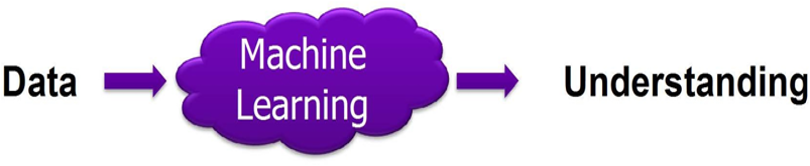
\includegraphics[width=14cm]{Images/AAv_Picture4.png}
\end{figure}
\end{frame}


\begin{frame}{{Problem Space}}
\begin{itemize}
    \item<2-> {\textbf{\textcolor{red}{Feature Extraction:}}} Find {\textcolor{red}{$x$}} corresponding to an  entity/item (such as an image, web page, ECG  etc.) Let us denote by {\textcolor{red}{$I$}}.
   \item<3-> {\textbf{\textcolor{red}{Classification:}}} Find a parameterized function which can make the right predictions.\\
   We denote the function by {\textcolor{red}{$f$}}. \\
   We denote the predictions by {\textcolor{red}{$y$}}.
   \item<4-> {\textbf{\textcolor{red}{End to End:}}} Can we learn {\textcolor{red}{$y$}} directly from {\textcolor{red}{$I$}}?
\end{itemize}
\end{frame}


\begin{frame}[t]{The Machine Learning Framework}
\vspace{-0.5cm}
\begin{figure} 
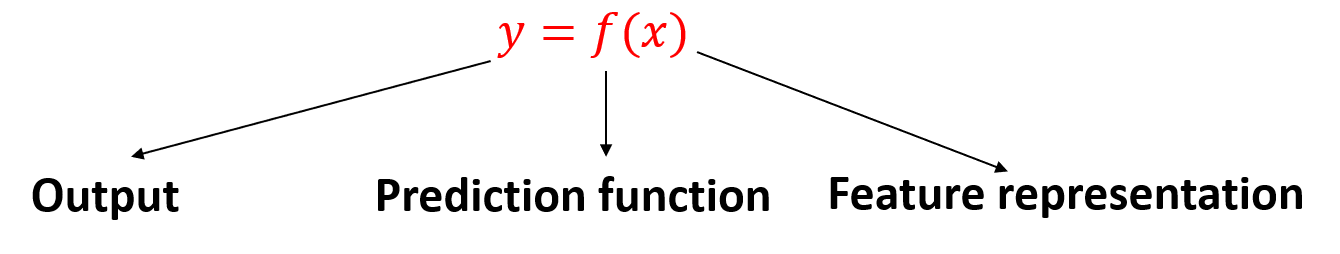
\includegraphics[width=10cm]{Images/AAv_Picture15.png} 
\end{figure}
\uncover<1->{\textbf{\textcolor{red}{Training:}} Given a training set, we estimate the prediction function, {\textcolor{red}{$f($ $)$}}, by minimizing the prediction error.}
	\\
\uncover<1->{\textbf{\textcolor{red}{Testing:}} Apply {\textcolor{red}{$f($ $)$}} to unknown test sample {\textcolor{red}{$x$}} and predicted value(output) is {\textcolor{red}{$y$}}}.
\end{frame}

\begin{frame}[t]{The Machine Learning Framework}
\vspace{-0.5cm}
\begin{figure} 
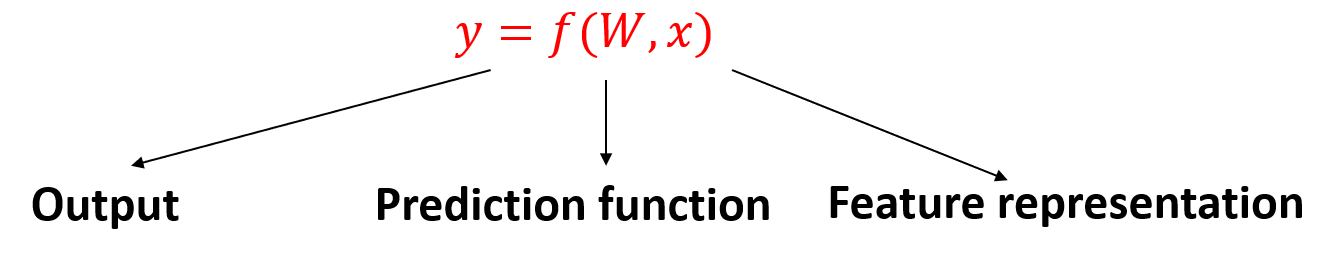
\includegraphics[width=10cm]{Images/AAv_Picture16.png} 
\end{figure}

{\textbf{\textcolor{red}{Training:}}} Given a training set, we estimate the prediction function, {\textcolor{red}{$f($ $)$}}, by minimizing the prediction error.
	\\
{\textbf{\textcolor{red}{Testing:}}} Apply {\textcolor{red}{$f(W,.)$}} to unknown test sample {\textcolor{red}{$x$}} and predicted value(output) is {\textcolor{red}{$y$}}.
\\~\\
{\textbf{\footnotesize{{\textcolor{red}{Parameter: Primary problem is to find the parameters,}}}{\textcolor{red}{$W$}}}}
\end{frame}

\begin{frame}
\frametitle{Spam Detection}
\centering
	\includegraphics<2>[width=15cm]{Images/AAv_Picture5.png}

\end{frame}

\begin{frame}
\frametitle{Spam Detection}
\begin{figure}
	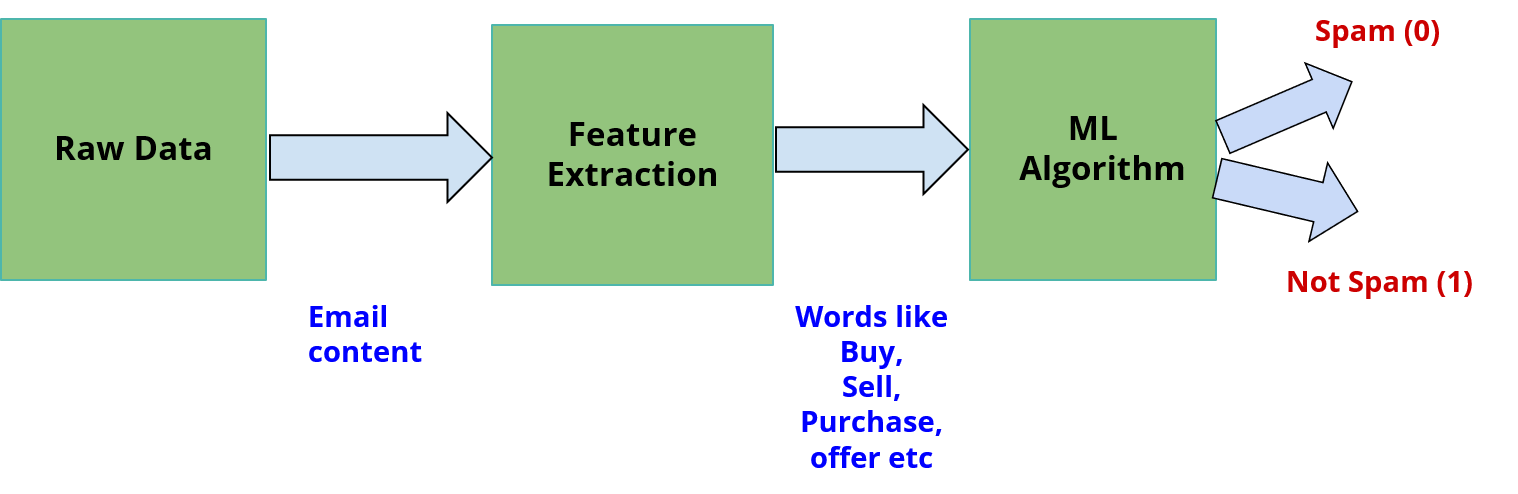
\includegraphics[width=15cm]{Images/AAv_Picture6.png}
\end{figure}
\end{frame}

\begin{frame}
\frametitle{Medical Diagnosis}
\begin{figure}
	\includegraphics<2>[width=15cm]{Images/AAv_Picture7.png}
\end{figure}
\end{frame}

\begin{frame}
\frametitle{Medical Diagnosis}
\begin{figure}
	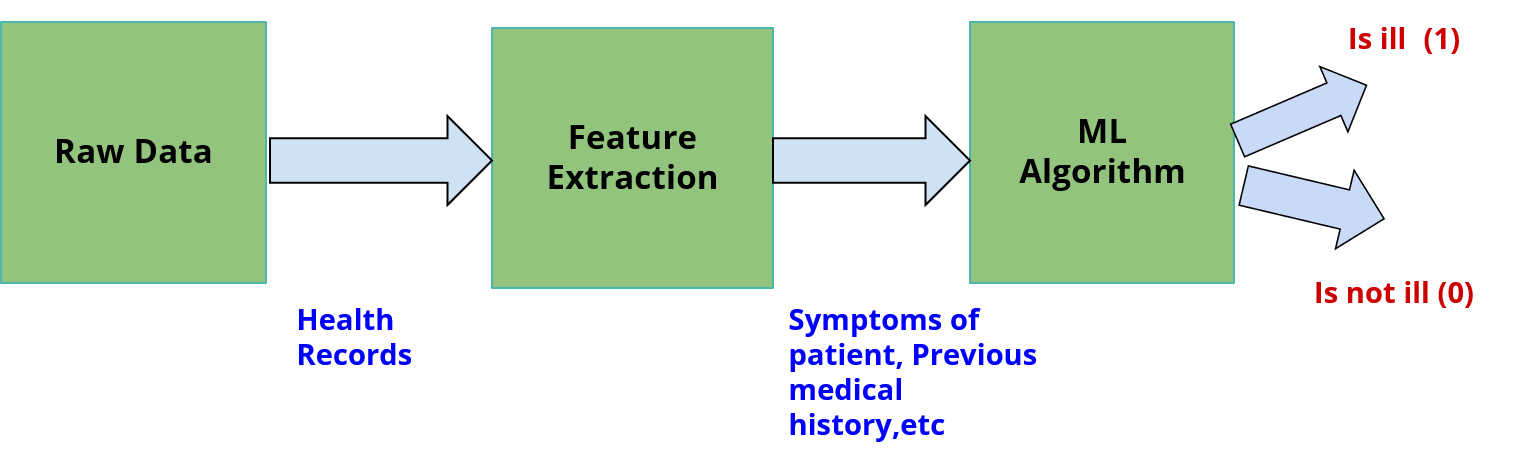
\includegraphics[width=15cm]{Images/AAv_Picture8.png}
\end{figure}
\end{frame}

\begin{frame}
\frametitle{Stock Trading}
\begin{figure}
	\includegraphics<2>[width=14cm]{Images/AAv_Picture9.png}
\end{figure}
\end{frame}

\begin{frame}
\frametitle{Stock Trading}
\begin{figure}
	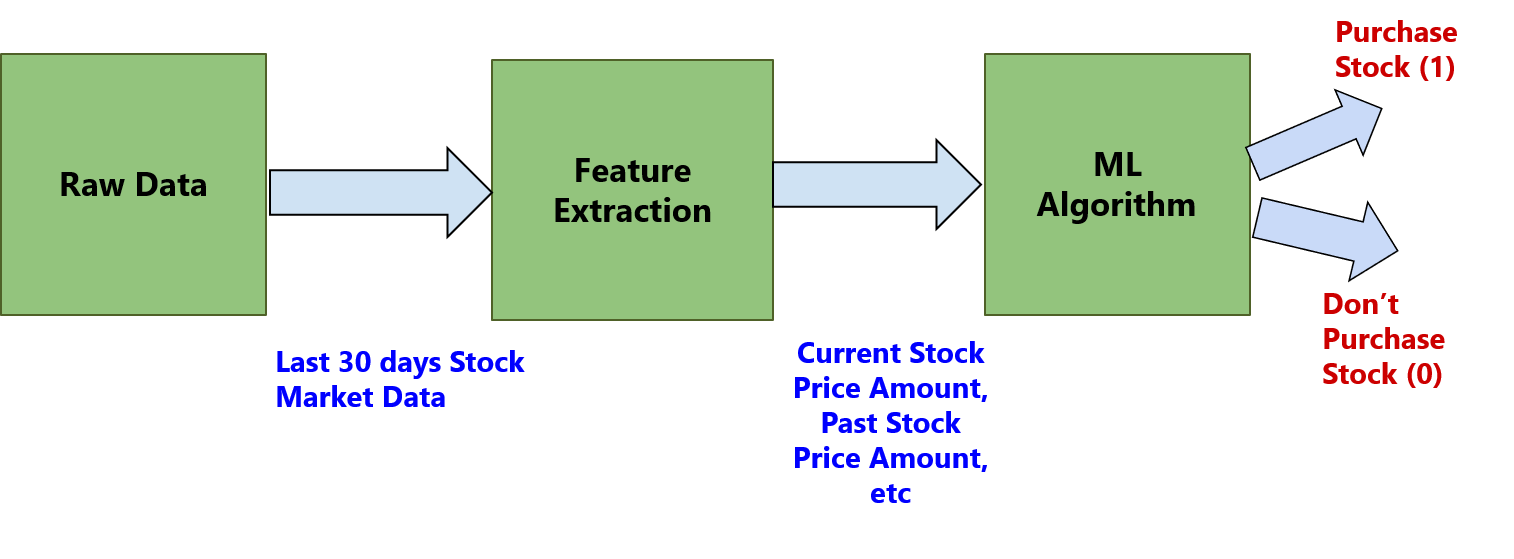
\includegraphics[width=14cm]{Images/AAv_Picture10.png}
\end{figure}
\end{frame}

\begin{frame}
\frametitle{Sentiment Analysis}
\centering
	\includegraphics<2>[width=15cm]{Images/AAv_Picture11.png}

\end{frame}


\begin{frame}
\frametitle{Sentiment Analysis}
\centering
	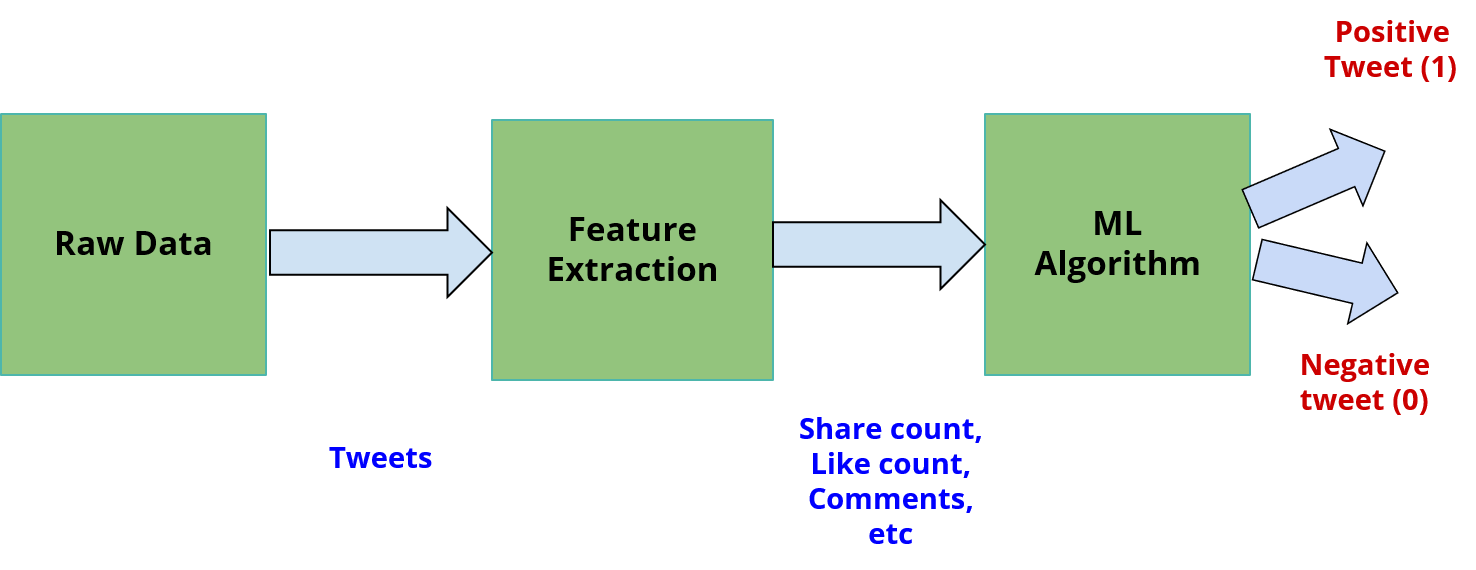
\includegraphics[width=15cm,height=5cm]{Images/AAv_Picture12.png}

\end{frame}

\begin{frame}
\frametitle{Disease Confirmation}
\centering
	\includegraphics<2>[width=14cm]{Images/AAv_Picture13.png}

\end{frame}

\begin{frame}
\frametitle{Disease Confirmation}
\centering
	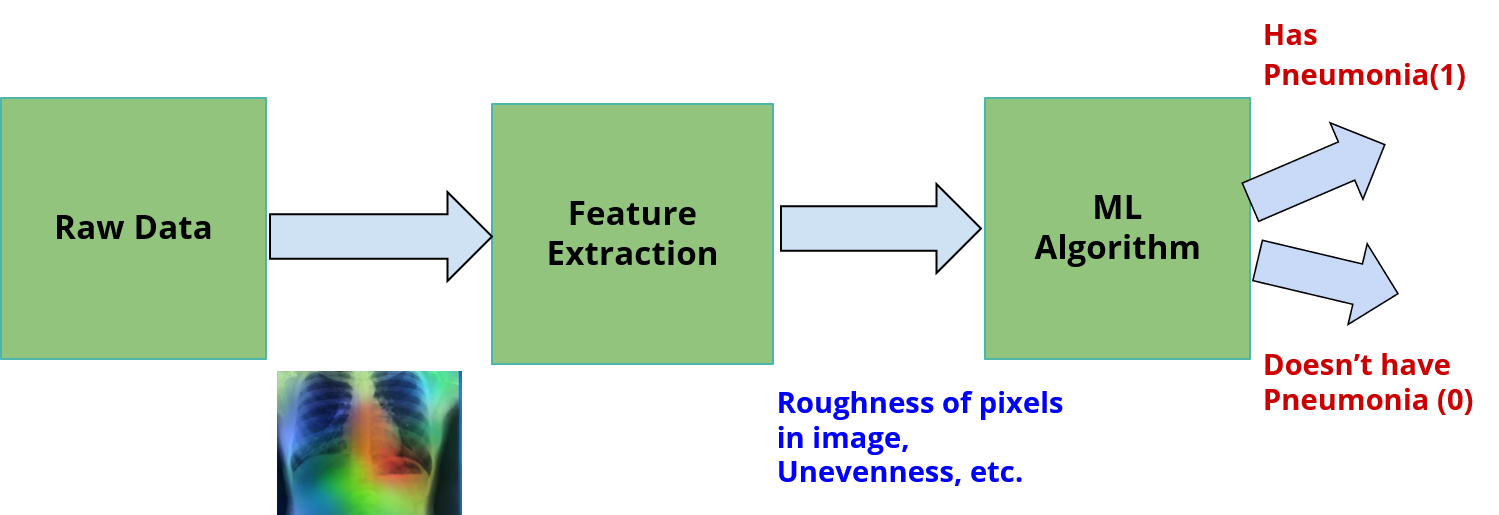
\includegraphics[width=15cm]{Images/AAv_Picture14.png}

\end{frame}


\begin{frame}
\frametitle{Product Recommendation}
\centering
	\includegraphics<2>[width=15cm]{Images/AAv_Picture17.png}

\end{frame}

\begin{frame}
\frametitle{Product Recommendation}
\centering
	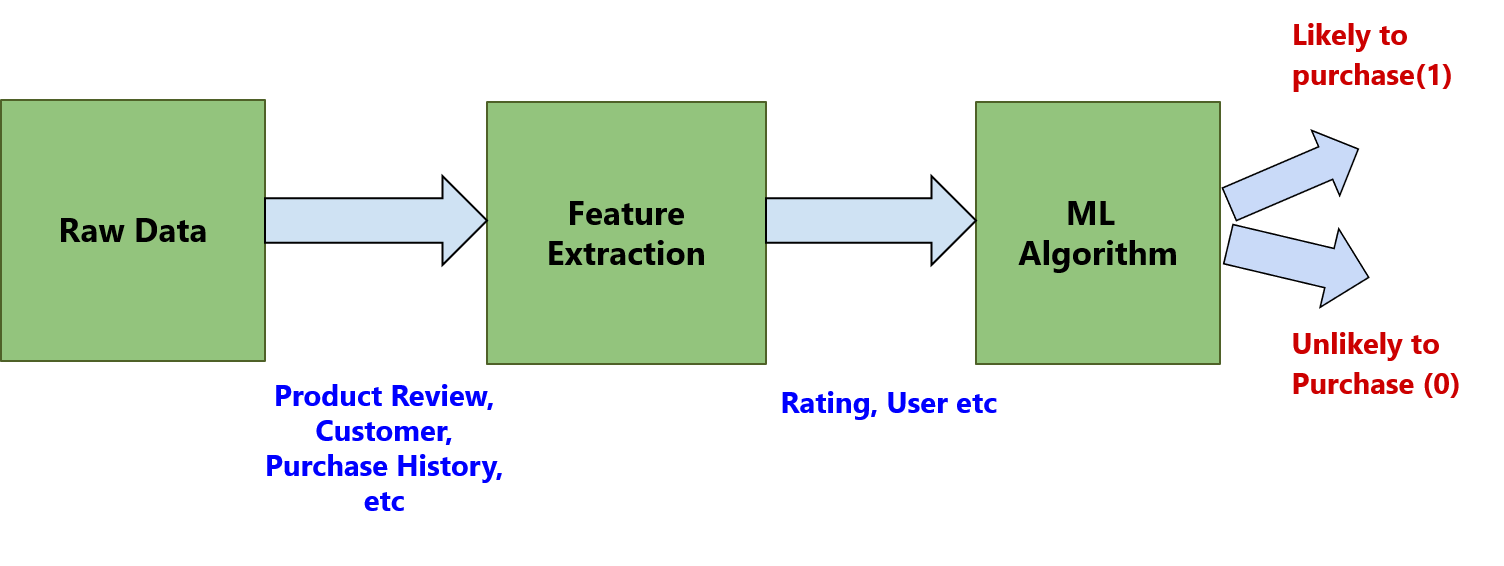
\includegraphics[width=15cm]{Images/AAv_Picture18.png}

\end{frame}


\begin{frame}
\frametitle{Loan Approval}
\centering
	\includegraphics<2>[width=15cm]{Images/AAv_Picture19.png}
\end{frame}

\begin{frame}
\frametitle{Loan Approval}
\centering
	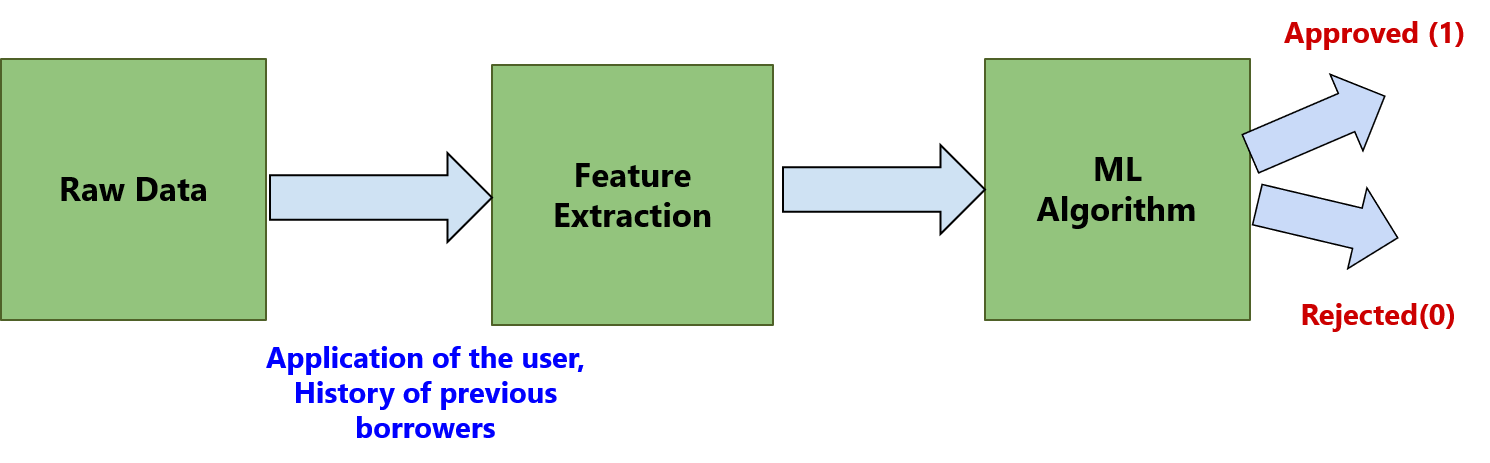
\includegraphics[width=15cm]{Images/AAv_Picture20.png}
\end{frame}

\begin{frame}
\frametitle{Face Recognition}
\begin{overlayarea}{14cm}{11cm}
	\includegraphics<2->[width=11cm]{Images/AAv_Picture21.png}

\includegraphics<3->[width=12cm]{Images/AAv_Picture21_1.png}
\end{overlayarea}
\end{frame}


\begin{frame}
\frametitle{Voice Detection}
\begin{overlayarea}{14cm}{11cm}
	\includegraphics<2->[width=11cm]{Images/AAv_Picture22.png}

\includegraphics<3->[width=12cm]{Images/AAv_Picture22_1.png}
\end{overlayarea}
\end{frame}



\begin{frame}
\frametitle{ML's Role in a Large Software System}
\begin{columns}
\column{0.65\paperwidth}
	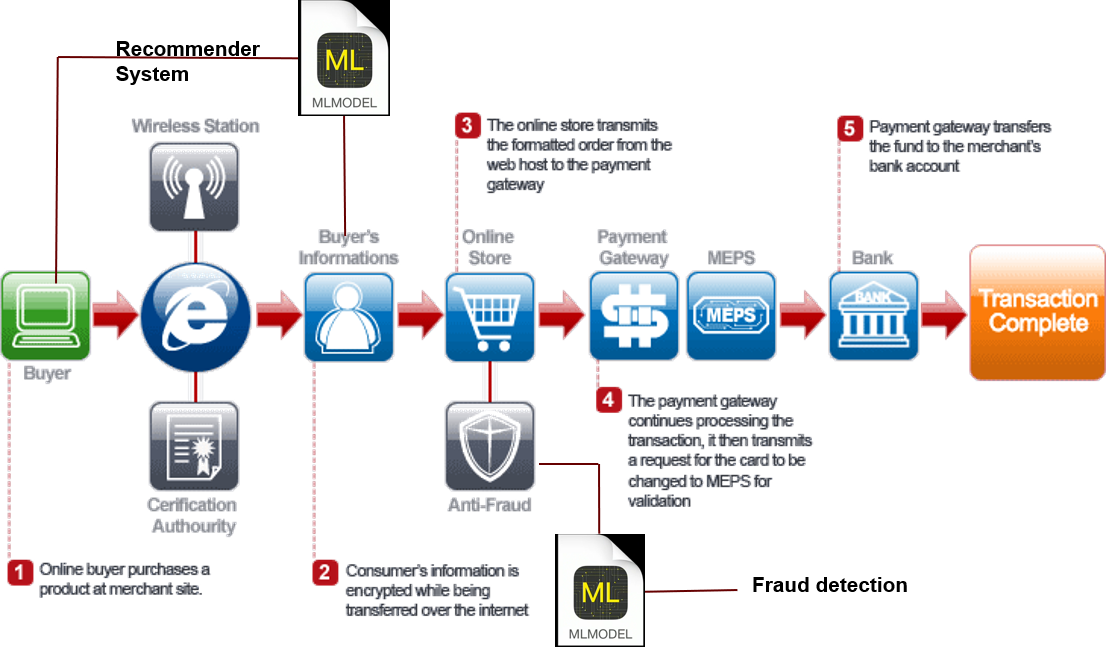
\includegraphics[width=10cm]{Images/AAv_Picture23.png}
\column{0.25\paperwidth}
\uncover<2->{ML can be considered as the \alert{“intelligent” block} in a large software system}
\end{columns}
\end{frame}

{\1
\begin{frame}[plain,noframenumbering]
 \centerpage{Thank you! \\ Questions?}
\end{frame}
}

\end{document}
